\section{A multi-view modeling framework} 

\begin{frame}{A multi-view modeling framework} 
  \begin{block}{Abstract}
    Acts as a background chapter about the models we use, their syntax and semantics. 
    Contributions shared with Damas thesis.
  \end{block}
  \begin{block}{Outline}
    \begin{itemize}
      \item Event-based Behavior Models
        \begin{itemize}
          \item Message Sequence Charts (MSC) for instance behaviors 
          \item Labeled Transition Systems (LTS) for class behaviors
        \end{itemize}
      \item State-based abstractions
        \begin{itemize}
          \item Capturing state information with Fluents
          \item Guards in behavior models
          \item Decorations on behavior models
        \end{itemize}
      \item Intentional models as goal graphs on fluents
        \begin{itemize}
          \item Goals and Fluent Linear Temporal Logic (FLTL)
          \item Linking FLTL and LTS: property and tester automata
        \end{itemize}
    \end{itemize}
  \end{block}
\end{frame}

\subsection{Event-based Behavior Models}

\begin{frame}{Message Sequence Charts for instance behaviors}
  \begin{center}
	  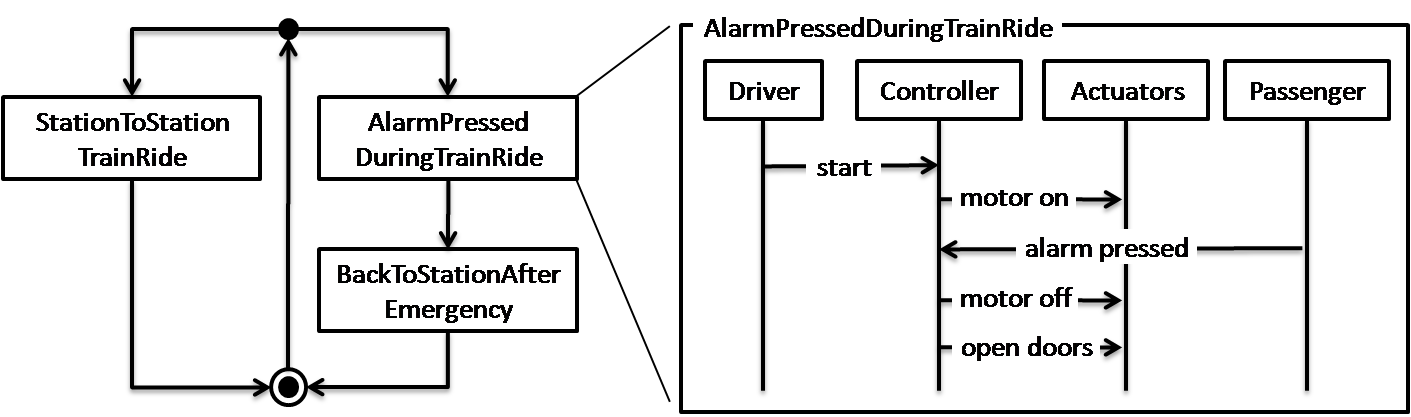
\includegraphics[width=12cm]{images/Train_hMSC_MSC.png}
  \end{center}
  \begin{block}{MSC (right) and high-level MSC (left)}
	  \begin{itemize}
		  \item Syntax of MSC and hMSC is described in \cite{ITU96}
		  \item Semantics of MSC and hMSC is defined in terms of Labeled Transition Systems, following \cite{Uchitel03}
		  \item We also allow a hMSC node to be refined as a finer-grained hMSC
	  \end{itemize}
  \end{block}
\end{frame}

\begin{frame}{Labeled Transition Systems for class behaviors}
  \vspace{-0.5cm}
  \begin{center}
	  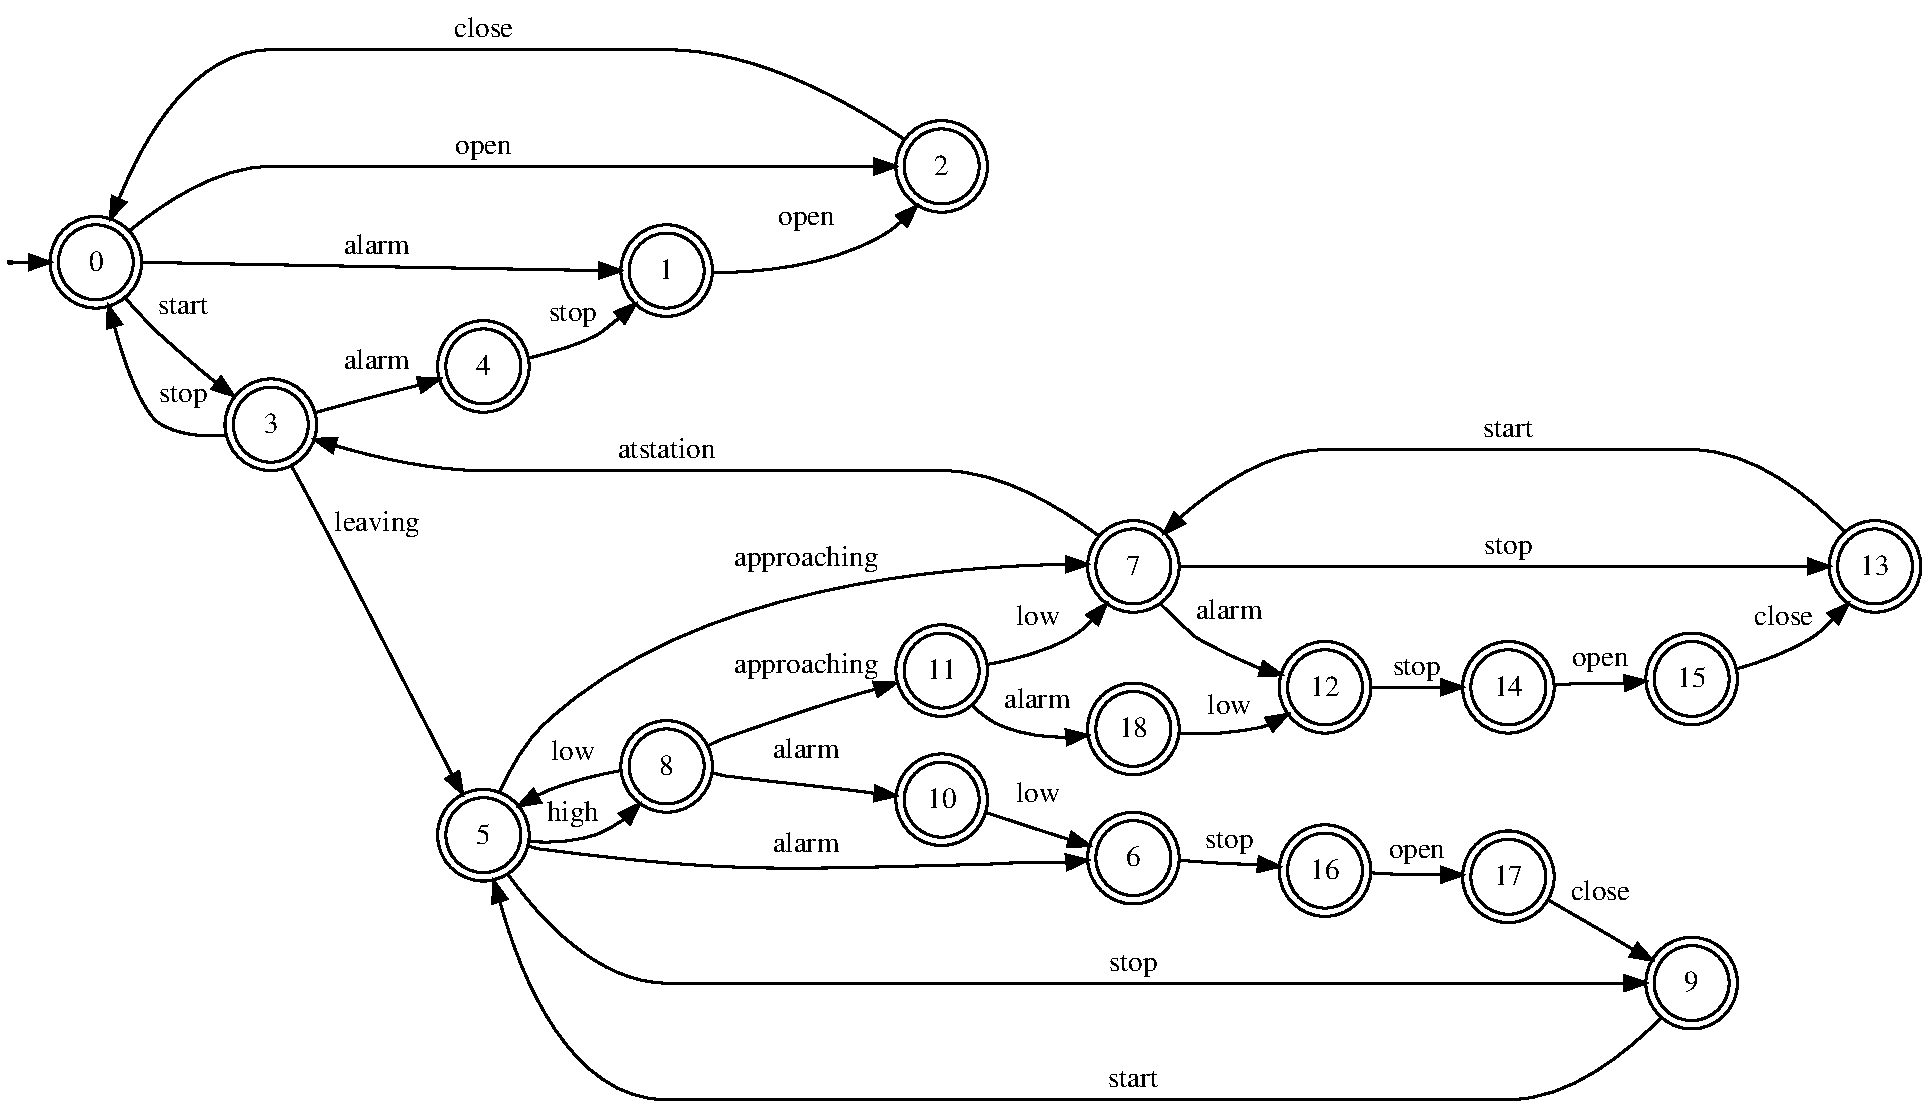
\includegraphics[width=10cm]{images/bigtrain.pdf}
  \end{center}
  \vspace{-1.5cm}
  \begin{block}{Labeled Transition Systems}
	  \begin{itemize}
		  \item Syntax and Semantics defined in \cite{Magee99}
		  \item Each agent behavior is defined by a LTS. The system behavior is defined by LTS composition
		  \item MSCs are admissible traces in the system LTS \cite{Uchitel03}
	  \end{itemize}
  \end{block}
\end{frame}

\subsection{State-based abstractions}

\begin{frame}{Capturing state information with Fluents}
  \begin{block}{Fluents capture the system state through the occurrence of events \cite{Milner89}}
	  \begin{center}
		  $fluent\;Fl = <init_{Fl}, term_{Fl}> initially\;Init_{Fl}$
	  \end{center}
	  \vspace{-0.4cm}
	  where $init_{Fl}$ and $term_{Fl}$ are disjoint set of events rendering the fluent $true$ and $false$, respectively
  \end{block}
  \begin{block}{Example}
	  \small
	  $fluent\;moving = <start, \{stop, emergency\;stop\}> initially\;false$
	  $fluent\;doors\_closed = <close, \{open, emergency\;open\}> initially\;true$
  \end{block}
\end{frame}

\begin{frame}{Guards in Behavior Models}
  \small
  \begin{block}{Summary}
	  Guards can be formally used in hMSC and LTS, leading to guarded hMSC (g-hMSC) and guarded LTS (g-LTS)
	  \begin{itemize}
	         \item A guard is a boolean expression on fluents
	         \item Structured forms for hMSC and LTS, avoiding state/trace explosion
	         \item Relax the assumption of fluent initial values being known for all instances
	  \end{itemize}
  \end{block}
  \begin{block}{Related publication}
	  \scriptsize
	  Damas C., Lambeau B., Roucoux F. and van Lamsweerde A., \emph{Analyzing Critical Process Models through Behavior Model Synthesis},
	  in Proc. ICSE'2009: 31th International Conference on Software Engineering, Vancouver, Canada, May 16-24, 2009. 
  \end{block}
\end{frame}

\begin{frame}{Guards in hMSC, i.e. g-hMSC}
  \begin{columns}
	  \column{.5\textwidth}
		  \begin{block}{Summary}
			  \begin{itemize}
				  \item \emph{Decision nodes}: outgoing transitions are labeled by boolean expressions on fluents
				  \item Initial condition $C_0$ stating an invariant on the initial state
				  \item Trace semantics through guarded LTS and LTS
				  \item Automated checking of guards: \emph{non overlapping}, \emph{completeness} and \emph{reachability}
			  \end{itemize}
		  \end{block}
	  \column{.5\textwidth}
		  \begin{center} 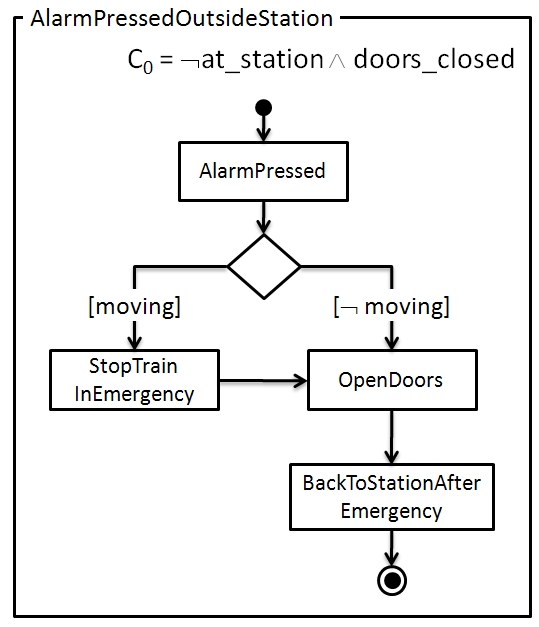
\includegraphics[width=5.5cm]{images/Train_guarded_hMSC.jpg} \end{center}
  \end{columns}
\end{frame}

\begin{frame}{Guards in LTS, i.e. g-LTS}
  \begin{block}{Summary}
	  \begin{itemize}
		  \item A g-LTS transition is labeled by an event or a guard
		  \item Initial condition $C_0$ stating an invariant on the initial state
		  \item A trace is accepted by a g-LTS if three conditions hold: \emph{trace inclusion}, \emph{admissible start} and \emph{guard satisfaction}
	  \end{itemize}
  \end{block}
  \begin{block}{Example}
	  \begin{center} 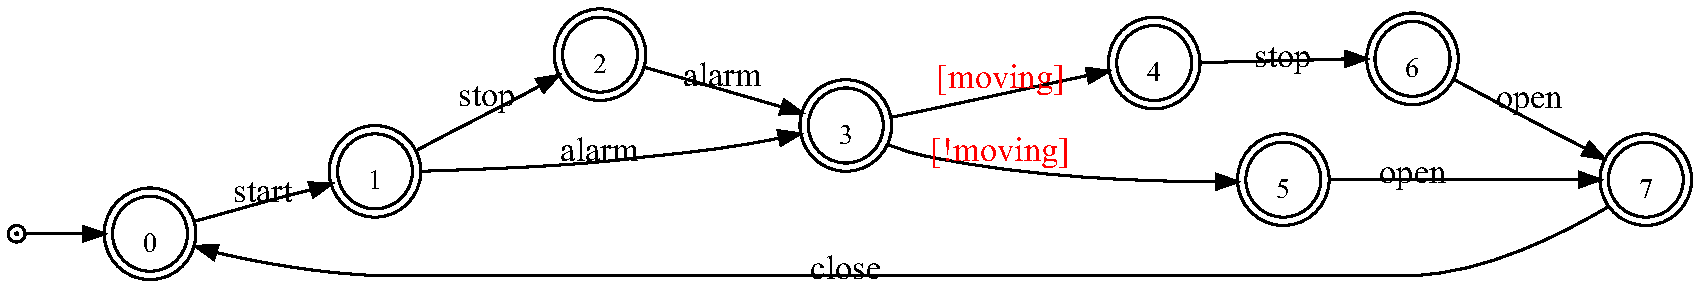
\includegraphics[width=11cm]{images/Train_guarded_LTS.pdf} \end{center}
	  \vspace{-0.5cm}
	  \begin{itemize}
		  \item $C_0 = \neg moving \wedge doors\_closed$
		  \item The event trace $(start\;alarm\;open)$ is not accepted due to the \emph{guard satisfaction} condition
	  \end{itemize}
  \end{block}
\end{frame}

\begin{frame}{Trace-based semantics of guarded LTS}

  A trace $(Init, <l_0,...>)$ is admitted from state $q_0$ by a guarded LTS $(Q,\Sigma,\Phi,\delta,q_0,C_0)$ iif 
  for every $i$, the following conditions hold
  
  \begin{itemize}
    \item trace inclusion:    $\exists q_{i+1} \in Q: (q_i,l_i,q_i+1) \in \delta$
    \item admissible start:   $Init \models C_0$
    \item guard satisfaction: $S_i \models l_i$ if $l_i \in 2^\phi$
  \end{itemize}
  
  where $S_i$ is the fluent value assignment after i-th event in the trace ($S_0 = Init$)

\end{frame}

\begin{frame}{Decorations on behavior models}
	\begin{block}{Summary}
		\begin{itemize}
			\item \cite{Damas05} proposes a decoration algorithm for generating fluent invariants on LTS states.
			\item In \cite{Damas10} the algorithm is generalized in order to 
				\begin{itemize}
					\item support additional decorations (e.g. cost, doses, time)
					\item support additional transition systems (guarded LTS in particular)
				\end{itemize}
		\end{itemize}
	\end{block}	
	\begin{block}{Example}
		\begin{center} 
			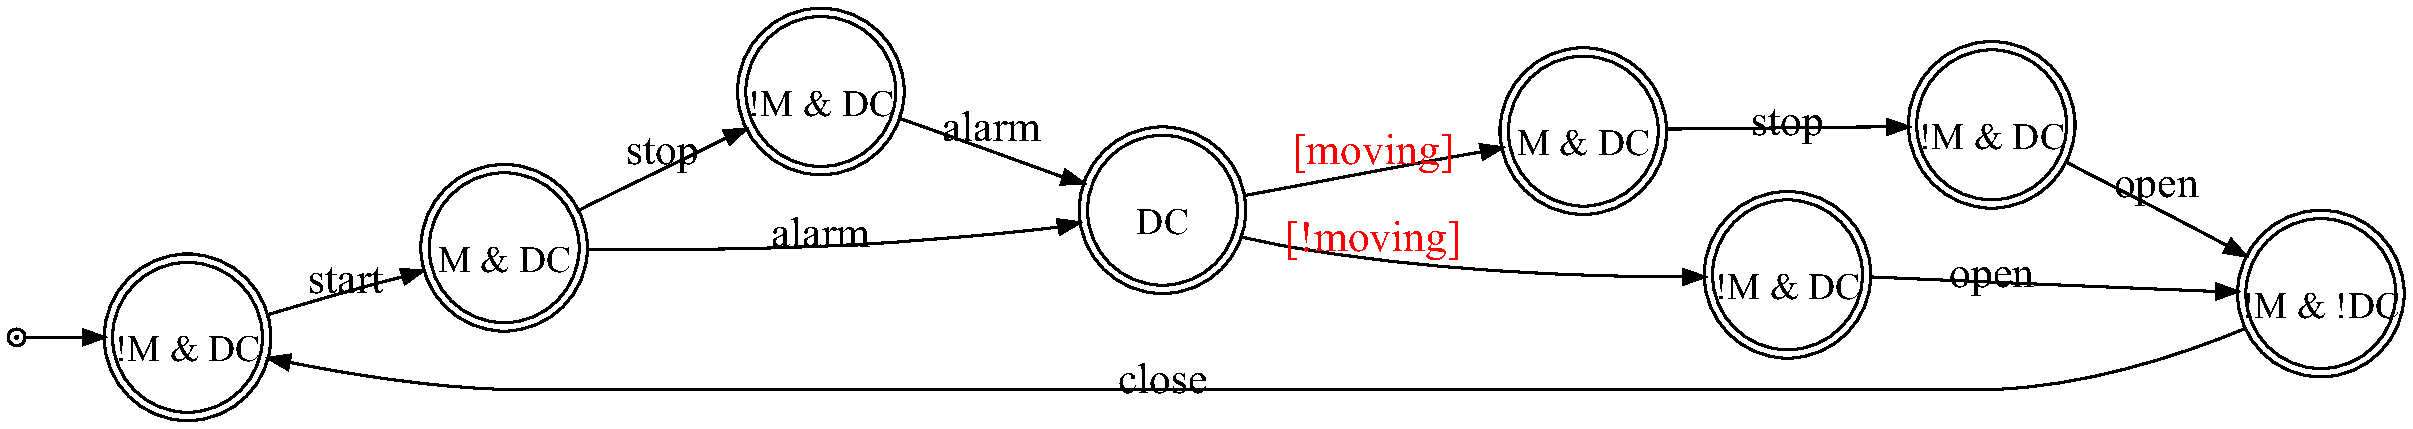
\includegraphics[width=11cm]{images/Train_guarded_LTS_decorated.pdf}
		\end{center}
		\vspace{-0.5cm}
		\begin{itemize}
			\item where $M$ stands for $moving$ and $DC$ stands for $doors\_closed$
		\end{itemize}
	\end{block}
\end{frame}

\subsection{Intentional models as goal graphs on fluents}

\begin{frame}{Intentional models as goal graphs on fluents}
	\begin{block}{Goals and Domain properties}
		\begin{itemize}
			\item Goals (resp. Domain properties) are prescriptive properties (resp. descriptive) about the system \cite{AVL09}
			\item Structured in AND/OR graphs
		\end{itemize}
	\end{block}
	\begin{block}{Fluent Linear Temporal Logic (FLTL)}
		\begin{itemize}
			\item Linear Temporal Logic \cite{Manna92} where propositions are Fluents
			\item FLTL is used in \cite{Gianna03} to model-check LTS against (state-based) temporal properties
		\end{itemize}
	\end{block}
	\begin{block}{Example}
		\begin{itemize}
			\item Maintain[DoorsClosedWhileMoving] : Train doors must always remain closed when the train is moving
			\item FormalDef: $\Box(moving \implies doors\_closed) $
		\end{itemize}
	\end{block}
\end{frame}

\begin{frame}{Linking FLTL and LTS}
	\begin{block}{Tester and Property LTS}
		\begin{itemize}
			\item A \emph{Tester LTS} can be synthesized from a FLTL safety property, as explained in \cite{Gianna03}. The error state
			          captures all event traces violating the property
			\item The \emph{Property LTS} obtained by removing the error state captures all event traces not violating the property \cite{Letier08}
		\end{itemize}
	\end{block}
	\begin{block}{Example}
		\vspace{-1cm}
		\begin{columns}
			\column{.5\textwidth}
				\begin{itemize}
					\item $\Box(moving \implies doors\_closed) $
				\end{itemize}
			\column{.5\textwidth}
				\begin{center} 
					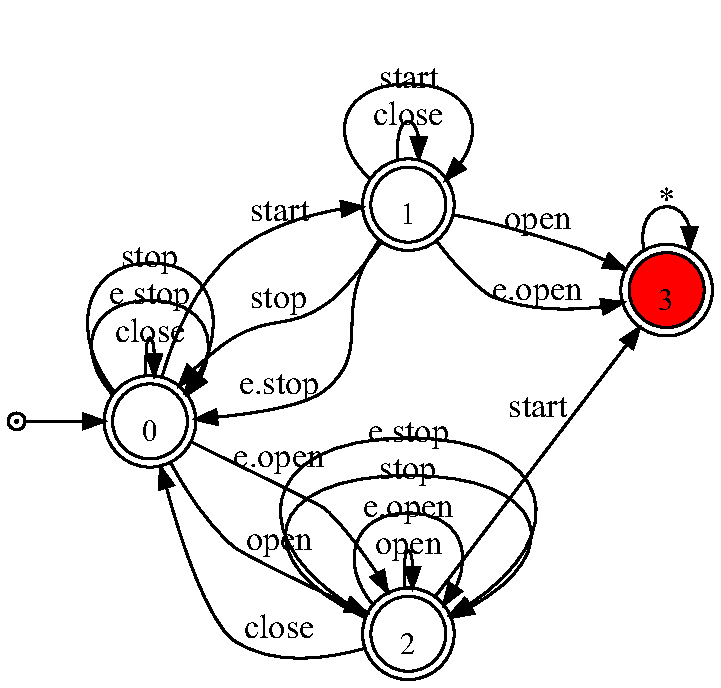
\includegraphics[width=4cm]{images/MaintainDoorsClosedWhileMoving.pdf}
				\end{center}
		\end{columns}
	\end{block}
\end{frame}


